\documentclass{article}
\usepackage{tenor2015}
\usepackage{times}
\usepackage{ifpdf}
\usepackage[english]{babel}
\usepackage{cite}
\usepackage{microtype}

\usepackage{inconsolata}
\usepackage{verbatim}

\usepackage{listings}
\lstset{language=Python,
showspaces=false,
showtabs=false,
breaklines=false,
showstringspaces=false,
breakatwhitespace=false,
escapeinside={(*@}{@*)},
keywordstyle=\bfseries,
basicstyle=\scriptsize\ttfamily
}

\def\papertitle{The design priorities behind Abjad:
Architecting an open-source software system for Formalized Score Control}
\def\firstauthor{Trevor Ba\v{c}a}
\def\secondauthor{Josiah Wolf Oberholtzer}
\def\thirdauthor{Jeffrey Trevi\~{n}o}
\def\fourthauthor{V\'{i}ctor Ad\'{a}n}

\newif\ifpdf
\ifx\pdfoutput\relax
\else
   \ifcase\pdfoutput
      \pdffalse
   \else
      \pdftrue
\fi

\ifpdf % compiling with pdflatex
  \usepackage[pdftex,
    pdftitle={\papertitle},
    pdfauthor={\firstauthor, \secondauthor, \thirdauthor, \fourthauthor},
    bookmarksnumbered, % use section numbers with bookmarks
    pdfstartview=XYZ % start with zoom=100% instead of full screen; 
                     % especially useful if working with a big screen :-)
   ]{hyperref}
  %\pdfcompresslevel=9

  \usepackage[pdftex]{graphicx}
  % declare the path(s) where your graphic files are and their extensions so 
  %you won't have to specify these with every instance of \includegraphics
  \graphicspath{{./figures/}}
  \DeclareGraphicsExtensions{.pdf,.jpeg,.png}

  \usepackage[figure,table]{hypcap}

\else % compiling with latex
  \usepackage[dvips,
    bookmarksnumbered, % use section numbers with bookmarks
    pdfstartview=XYZ % start with zoom=100% instead of full screen
  ]{hyperref}  % hyperrefs are active in the pdf file after conversion
  \usepackage[dvips]{epsfig,graphicx}
  \graphicspath{{./figures/}}
  \DeclareGraphicsExtensions{.eps}
  \usepackage[figure,table]{hypcap}
\fi

\hypersetup{
    colorlinks,
    citecolor=black,
    filecolor=black,
    linkcolor=black,
    urlcolor=black
}

%\title{\papertitle}
\title{The design priorities behind Abjad: \\ 
Architecting an open-source software system \\
for Formalized Score Control}

\fourauthors
  {\firstauthor} {Harvard University \\
    {\tt \href{mailto:trevor.baca@gmail.com}
        {trevor.baca@gmail.com}}}
  {\secondauthor} {Harvard University \\
    {\tt \href{mailto:josiah.oberholtzer@gmail.com}
        {josiah.oberholtzer@gmail.com}}}
  {\thirdauthor} {Carleton College \\
    {\tt \href{mailto:jeffrey.trevino@gmail.com}
        {jeffrey.trevino@gmail.com}}}
  {\fourthauthor} { 
    {\tt \href{mailto:vctradn@gmail.com}
        {vctradn@gmail.com}}}

\begin{document}

\capstartfalse
\maketitle
\capstarttrue

\begin{abstract}
Abjad\footnote{www.projectabjad.org} is an interactive open-source software
system designed to help composers build up complex pieces of music notation in
an iterative and incremental way.  Abjad is implemented in the
Python\footnote{www.python.org} programming language and architected as an
object-oriented collection of packages, classes and functions. Composers can
visualize their work as publication-quality score at all stages of the
compositional process using Abjad's interface to the
LilyPond\footnote{www.lilypond.org} music notation package. Although the first
versions of Abjad were implemented in 1997 and the project website is now
visited thousands of times each month, we have never documented the design
priorities that have guided us as we have built the system. In this paper we
detail some of the most important principles we have followed in our work
architecting Abjad. The priorities we document here arise in answer to
domain-specific questions of music modeling (what are the fundamental elements
of music notation? which elements of music notation should be modeled
hierarchically? which programming constructs are available to help model the
temporal relationships arising between entities in musical score?) as well as
in consideration of the ways in which best practices taken from software
engineering can apply to the development of a music software system like ours
(which programming concepts concerning things like iteration, aggregation and
encapsulation make sense to make available to composers? which existing tools
to test, document and deploy other open-source projects are available to help
develop a music software system like Abjad?). In the sections that follow we
discuss the background and motivations that lead us to ask questions like these
and then elaborate the design priorities we have arrived at in our ongoing work
architecting Abjad.
\end{abstract}

\section{Background \& Motivations}\label{sec:background}

While many environments for both notation and sound production have arisen
within the last twenty years, the following discussion focuses solely on the
production of notation: Abjad enables composers to express both low- and
high-level compositional ideas by extending a widely used programming language
to provide a sufficiently detailed object model of common practice musical
notation. To minimize the restriction of artistic thought's infinite
possibility while maximizing the ability to specify elegantly any arbitrary
symbolic relationship, Abjad does this without prescribing explicit or implicit
models of music or composition: Abjad defines composition narrowly as the act
of creating a document via the encoded aggregation of notational symbols.

\subsection{Generative Task as an Analytic Framework}

Software production exists as an organizationally designed feedback loop
between production values and implementation \cite{Derniame:1999fk}, and it is
possible to understand a system by understanding the purpose for which it was
initially designed, the system's \emph{generative task(s)}. In the analysis of
systems created for use by artists, this priority yields a dilemma instantly,
as analyses that explain a system's affordances with reference to intended
purpose must contend with the creative use of technology by artists: a system's
intended uses might have little or nothing in common with the way in which the
artist finally uses the technology. For this reason, the notion of generative
task is best understood as an explanation for a system's affordances, with the
caveat that a user can nonetheless work against those affordances to use the
system in novel ways. Generative tasks --- informed by the cultural milieu of
software development, economic constraints of software production, and the
aesthetic proclivities of artists participating in development processes ---
constrain software features to enable a limited subset of possible
representations and user interactions.

While composers working traditionally may allow intuition to substitute for
formally defined principles, a computer demands the composer to think formally
about music \cite{Xenakis:1992rq}. Keeping in mind generative task as an
analytical framework, it is broadly useful to bifurcate an automated notation
system's development into the modeling of music and composition, on the one
hand, and the modeling of musical notation, on the other. All systems model
both, to greater or lesser degrees, often engaging in the ambiguous or implicit
modeling of music and composition while focusing more ostensibly on a model of
notation, or focusing on the abstract modeling of music without a considered
link to a model of notation. Due to the intimate link between notation and
musical ideas, it is impossible for a system that models notation to avoid at
least implicitly modeling musical and compositional ideas, and a computational
model of music and composition is an inevitable component of every automated
notation system, even when it exists as an unspoken set of technological
constraints. Generative task explains a given system's balance between
computational models of music/composition and notation by assuming a link
between intended use and system development.

\subsection{Computational Models of Notation}

Many systems implement detailed models of music explicitly or implicitly, but
few of these implement detailed models of notation.\footnote{Computational
models of music might entail the representation of higher-level musical
entities apparent in the acts of listening and analysis but absent in the
symbols of notation themselves, as determined to be creatively exigent.
Programming researchers and musical artists have modeled many such
extrasymbolic musical entities, such as large-scale form and transition
\cite{polansky1991morphological}, \cite{uno1994temporal},
\cite{dobrian1995algorithmic}, \cite{abrams1999higher}, \cite{Yoo1983}, texture
\cite{Horenstein:2004kx}, contrapuntal relationships \cite{Boenn:2009oq},
\cite{Acevedo2005}, \cite{Anders:2011kl}, \cite{Balser:1990tg},
\cite{Jones:2000hc}, \cite{uno1994temporal}, \cite{Bell:1995ij},
\cite{farbood2001analysis}, \cite{Cope:2002fv}, \cite{Laurson:2005dz},
\cite{Polansky:2011fu}, \cite{Ebcioglu:1980kl}, harmonic tension and resolution
\cite{Melo2003}, \cite{Wiggins1999}, \cite{Foster:1995qa}, melody
\cite{Hornel:1993mi}, \cite{Smith:1992pi}, meter \cite{Hamanaka:2005ff}, rhythm
\cite{Nauert2007}, \cite{Degazio:1996lh}, \cite{Collins:2003bs}, timbre
\cite{Xenakis:1991fu}, \cite{Creasey:1996ye}, \cite{Osaka2004}, temperament
\cite{Seymour:2007qo}, \cite{Graf:2006il}, and ornamentation
\cite{Ariza:2003zt}, \cite{Chico-Topfer:1998jl}. This work overlaps fruitfully
with analysis tasks, and models of listening and cognition can enable novel
methods of high-level musical structures and transformations, like dramatic
direction, tension, and transition between sections \cite[108]{Collins2009}.} A
system that affords a detailed model of music/composition without linking to a
sufficiently detailed model of musical notation does not afford automated
notation --- sufficiency, however, depends heavily on generative task. For
example, if a composer requires an automated notation system to render complex
rhythmic ideas that depend typographically on nested tuplets, a system that
produces a notation only via a combination of MIDI and quantization must reduce
rhythms to a non-hierarchical stream of event times, eliminating the temporally
divisive approach of tuplet notation. For many rhythmic applications, though,
MIDI suffices. 

Many automated notation systems exist to model musical notation and the act of
typographical layout without explicitly affording the computational modeling of
music or composition \cite{Smith:1972mw}, \cite{Nienhuys:2003ve},
\cite{Hoos:1998bd}, \cite{hamel1noteability}; many of these systems strongly
imply a model of music, such as Gr\'{e}goire for Gregorian chant, Django for
guitar tablature, and GOODFEEL for Braille notation \cite{2006}, while
feature-rich systems (often oriented toward classical composers) such as
Finale, Sibelius, SCORE, Igor, Berlioz, and Nightingale, present themselves as
relatively more genre-agnostic software tools. Such a system might go so far as
to enable a text-based object-oriented model of notation that automates some
aspect of an otherwise point-and-click interface, as in the case of Sibelius's
ManuScript scripting language \cite{Technology:qc}. 

Many models of musical notation have been designed created for purposes of
corpus-based computational musicology. Formats such as Music21, DARM, SMDL,
HumDrum, and MuseData model notation with the generative task of searching
through a large amount of data \cite{Selfridge-Field:1997ud}. Commercial
notation software developers attempted to establish a data interchange standard
for optical score recognition (NIFF) \cite{niff1995niff}; since its release in
2004, MusicXML has become a valid interchange format for over 160 applications
and maintains a relatively application-agnostic status, as it was designed with
the generative task of acting as an interchange format between variously tasked
systems \cite{Good:2001if}. (are Igor and Berlioz commercial?)

Notation representations that underly many of these GUI-based systems often go
undescribed as computer representations of notation, in favor of discussions
about human-computer interaction. For example, Barker and Cantor developed an
early model of music notation that underlies a four-oscilloscope GUI and
describe their work entirely in terms of user interaction
\cite{cantor1971computer}; likewise, discussions of modern commercial notation
systems remain similarly oriented, without much awareness or criticism of the
underlying computational models of notation. This results in insufficiently
detailed models of notation; systems, for example, that provide models only of
mensural notation and enable nonmensural notations only as modified
instantiations of notations based on measures.

\subsection{The Development of Hierarchical Object Models of Notation}

Many early models of musical notation were not hierarchical, and Lejaran
Hiller, in reflecting on decades of automated notation work, identifies the
lack of hierarchical organization as a limitation of early work --- although
Nick Collins points out that even Hiller's program PHRASE addresses the
hierarchical organization of a score up to the level of a phrase, without
moving beyond this mid-level musical structure to concerns of large-scale form
\cite[108]{Collins2009}. 

There were several object-oriented music environments by 1990
\cite[139]{Polansky:1990fk}, most created in or inspired by the newly popular
Smalltalk-80 programming language; while they facilitated the hierarchical
modeling of musical abstractions, they omitted or radically simplified the
hierarchical nature of common notation. For example, Glen Krasner (Xerox
Systems Science Laboratory) created Machine Tongues VIII, a music system that
created an object-oriented model of the score/orchestra distinction inherited
from Max Mathews' Music N languages, with a simple linear model of ``partOn''
and ``partOff'' command sequences \cite{Krasner:1991uq}, omitting hierarchical
organization entirely when the system produced notational output; although
subsequent Machine Tongues systems introduced some hierarchical organization
via ``note'' objects that inhabited ``event lists,'' systems did not attempt to
model the hierarchical detail of all a traditional score's elements. Like
Hiller's PHRASE program, Andreas Mahling's CompAss system organized events
hierarchically up to the mid-level ``phrase'' level of musical structure
\cite{Mahling:1991qf}. These systems extend Smalltalk-80 with interfaces to the
MIDI communications protocol: as extensions of Smalltalk, they enabled the user
to arbitrarily extend the system with new objects, creating a detailed and
hierarchical model of music, usually flattened into a list of noteOn and
noteOff commands to be notated or played back via MIDI interface. 

By 1989, Glendon Diener's Nutation system (written in Objective C for the NeXT
computer) modeled both musical and notational structure hierarchically through
the use of directed graphs \cite{Diener:1991zr}, \cite{Diener:1991ly},
\cite{Diener:1989ve}.

last section: system motivations

Linking our design priorities with those of previous systems by describing
perceived deficiencies: evaluative priorities for previous systems: sufficiency
instead of comprehensiveness, potentially evaluated by sonic result rather than
notation, addressability (in HMSL and JMSL). Reintroduce generative task: late
50s through 80s were motivated locally by generative tasks of specific projects
until IRCAM's Patchwork approached a generative task of broadly enabling
composers; sufficiency determined by comprehensive task.

\section{Extend an existing language: \\ No domain-specific languages}

Abjad is not a programming langauge. Abjad instead extends the Python
programming language. Our insistence on this principle of extension --- of
adding functionality to an existing programming language rather than inventing
yet another domain-specific language --- originates in the belief that there is
no real benefit to be had in reestablishing the ways variables are created,
references are handled, loops are structured or any of the other fundamentals
of programming. We have instead architected Abjad in the form of a Python
package designed to be used the same way as the thousands of other packages
that equip Python with new functionality.\footnote{See the Python Package Index
for functionality to extend the language for purposes as diverse as creative
writing and aeronautical engineering. The Python Package Index contains 54,306
packages at the time or writing and is available at \textit{pypi.python.org}.}
In designing Abjad as an extension to a widely used language we make relevant
both the hundreds of already-available print and Web resources that detail
Python and its features as well as the global community of developers working
in the language. Both benefits we hope to ease composers' transition to
programming and make working with Abjad a familiar task that conforms to widely
understood programming best practices: there will probably by necessity always
be more programmers than composers in the world and it makes sense for our work
as composers to benefit from the patterns already understood elsewhere in the
culture.

Though we continue to find Python an excellent programming
language,\footnote{Aspects of Python we find particularly helpful include the
availability of lists, dictionaries and sets as built-in types; the interface
provided for string and Unicode objects; the unified approach to encapsulation
provided by Python's understanding of namespaces; and the extensive
functionality provided in the standard library.} our decision to implement
Abjad in Python does not arise from the specifics of the language but from the
large community of users the language supports and the fact that Python is open
source. The history of music software systems is littered with projects that
fell into disuse. Music software systems except for the large commercial
notation packages will probabaly always be the niche efforts of specialists and
our experience architecting Abjad leads us to think about the future in such a
way that we give ourselves all the advantages of expansiveness that are
possible: picking an existing language that makes learning preliminaries
easier and makes the continued development of the system as open as possible to
as many different collaborators as possible.

\section{Allow composers to illustrate objects iteratively during composition }

One of the core beliefs we bring to our work architecting Abjad concerns the
power of conventional music notation. We believe that it is important for
composers be able to illustrate the objects they work with as they compose.
This priority in favor of iteratively viewing the objects of composition is
reflected in the \emph{illustration protocol} \footnote{Python describes common
informal interfaces to working with objects as \emph{protocols}. Important
protocols include the \emph{iterator protocol} for iterating over the contents
of a container-like object, the \emph{sequence protocol} for getting items and
length from a container-like object and the \emph{mutable container protocol}
for mutating the contents of a container-like object.} established for Abjad
objects. Composers call the top-level \texttt{show()} function to visualize
Abjad objects. Behind the scenes Abjad inspects objects passed to
\texttt{show()} for the presence of an \texttt{\_\_illustrate\_\_()} method
that defines explicitly how an object should be illustrated. Abjad transforms
score components, for example, into LilyPond input code and then calls LilyPond
to generate a PDF that is then pushed to the composer's PDF viewer.

%priority is driven in large part by our shared insistence on the incredible
%power of conventional music notation as a tool for thinking about sound and
%time. (we wanna make it possible to illustrate everything all the time because
%we notation helps us think about such incredibly complex stuff.) (footnote: we
%think it's important that users have access to all the features of the
%underlying typesetter.) [TREVOR]

%We believe that the objects that composers work with should all theoretically
%be viewable as notation. To this end Abjad makes visualizing notational
%artifacts simple. Any notational element or element aggregate can be displayed
%at any time as a PDF by calling the top-level \texttt{show()} function. The
%motivation of the principle is immediate when discussing classes like
%\texttt{Note}, \texttt{Rest} and \texttt{Chord} that model printed symbols on
%the page. But Abjad invites developers and advanced users to extend the
%principle of notational reality to include the abstract relationships in which
%music and music composition are rich: users can call \texttt{show()} on
%abstract objects like the Abjad \texttt{Duration}\footnote{Also
%\texttt{PitchClass}, \texttt{Mode}, \texttt{Scale} and many other classes.}
%class to view any duration as a typeset fraction. The decision to notate
%durations this way is wholly conventional but increases the extent to which
%users can feel confident that they will be able to view the objects they
%create. The same is true of many other Abjad classes that model abstract
%relationships: \texttt{Mode}, \texttt{Scale}, \texttt{PitchClass} and so on.

%For example, Abjad expresses the durations of all score components in terms of
%rational values -- fractions and integers -- rather than floating point
%numbers. Likewise Abjad expresses all pitches in terms of triples of diatonic
%note names, accidentals and octave numbers, rather than MIDI numbers or
%frequencies. While Abjad provides alternative representations of pitch and
%rhythm, as well as affordances for moving between them, the format actually
%stored in and used by score components for rendering notation is always the
%most notationally-explicit.

\section{Bottom-up construction}

It's important for composers to be able to build complex score bottom-up.

Abjad affords aggregation via Python's \emph{mutable sequence} protocol, a
collection of instance methods which allow score components to be appended,
extended or inserted into other container-like score components as though they
were lists.

Abjad assumes notational primitives are the elements of composition.

The act of composition then revolves around the iterative aggregation of
notational primitives into arbitrarily complex score objects.

Input flexibility.

You can build up score via iterative aggregation but you can also just type a
lilypond string into a staff.

We afford both types of input and, indeed, two different ways of building up
score.

This is where we should cite alan kay's smalltalk paper.

("it's easy to make a thing.")

We make it easy to build up complex score objects through iterative
aggregation.

("we make it easy to build things up.")

[JOSIAH]

\begin{lstlisting}
>>> outer_tuplet_one = Tuplet((2, 3), "d''16 ef'8.")
>>> inner_tuplet = Tuplet((4, 5), "cs''16 e'16 d'2")
>>> outer_tuplet_one.append(inner_tuplet)
>>> outer_tuplet_two = Tuplet((4, 5))
>>> outer_tuplet_two.extend("d'8 r16 b'16 as'16")
>>> tuplets = [outer_tuplet_one, outer_tuplet_two]
>>> upper_staff = Staff(tuplets, name='Upper Staff')
>>> upper_staff.extend("as'8.. fs'32")
>>> lower_staff = Staff(name='Lower Staff')
>>> lower_staff.extend("c8 r8 b8 r8 gf8 r4 cs8")
>>> staff_group = StaffGroup()
>>> staff_group.extend([upper_staff, lower_staff])
>>> score = Score([staff_group])
>>> show(score)
\end{lstlisting}

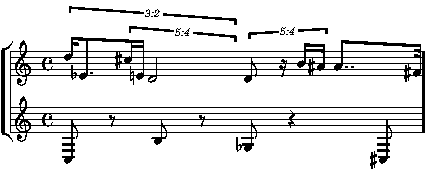
\includegraphics[scale=1.0]{images/abjad-1.pdf}


\begin{lstlisting}
>>> upper_leaves = upper_staff.select_leaves()
>>> lower_leaves = lower_staff.select_leaves()
>>> attach(Tie(), upper_leaves[4:6])
>>> attach(Tie(), upper_leaves[-3:-1])
>>> attach(Slur(), upper_leaves[:2])
>>> attach(Slur(), upper_leaves[2:6])
>>> attach(Slur(), upper_leaves[7:])
>>> attach(Clef('bass'), lower_leaves[0])
>>> show(score)
\end{lstlisting}

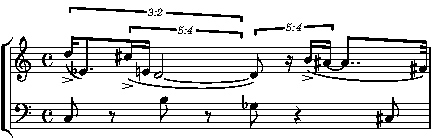
\includegraphics[scale=1.0]{images/abjad-2.pdf}


\section{Top-down construction}

it's important for composers to be able to build complex
score top-down.

we provide factories, factory functions, factory classes.

when we wanna make complex stuff we usually come up with factories.

(there may be a design principle here that initialization is kept simple and we
implement in factories complex ways of aggregating together objects that admit
only simple initialization.)

(we generalize many of these things in processes.)

there's a design priority in here somewhere that what we want to do is make it
as easy as possible for people to implement their own factories.

what does this mean? it means that we want to make it as easy as possible for
people to implement their own code that outputs or creates intermediate level
structures or materials.

(there's a realization here that people probabaly don't find it interesting to
make a single note. but people can find it totally fascinating to make an
intermediate-level object like a complete phrase of music.)

we think it's important for composers to be able to create their own processes
that generalize these things.

with experience, use of the system migrates from bottom-up to top-down: just
look at us! this is what is closest to the work of beginning to implement one's
own system of composition.

this is where we make the case for esthethic-agnositicism.

this is also an important point about extensibility.

rhythm makers, score templates, etc.

\begin{lstlisting}
>>> divisions = [(3, 8), (5, 16), (1, 4), (5, 16)]
>>> rhythm_maker = rhythmmakertools.NoteRhythmMaker()
>>> show(rhythm_maker, divisions=divisions)
\end{lstlisting}

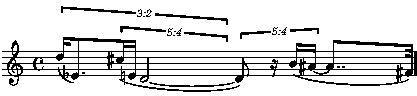
\includegraphics[scale=1.0]{images/abjad-3.pdf}


\begin{lstlisting}
>>> rhythm_maker = rhythmmakertools.TaleaRhythmMaker(
...     extra_counts_per_division=(0, 1, 1),
...     talea=rhythmmakertools.Talea(
...         counts=(1, 2, 3),
...         denominator=16,
...         ),
...     )
>>> show(rhythm_maker, divisions=divisions)
\end{lstlisting}

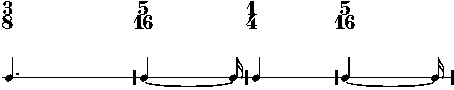
\includegraphics[scale=1.0]{images/abjad-4.pdf}


\begin{lstlisting}
>>> template = templatetools.GroupedRhythmicStavesScoreTemplate(4)
>>> quartet_score = template()
>>> iterator = iterate(quartet_score).by_class(Voice)
>>> for index, voice in enumerate(iterator):
...     divisions = sequencetools.rotate_sequence(
...         divisions, -1)
...     selections = rhythm_maker(divisions, seeds=index)
...     measure = Measure((5, 4), selections)
...     voice.append(measure)
... 
>>> show(quartet_score)
\end{lstlisting}

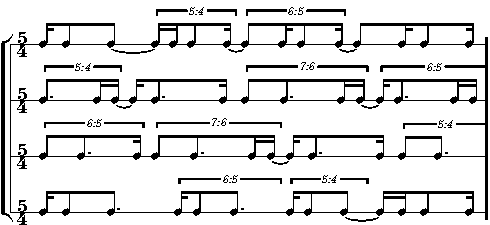
\includegraphics[scale=1.0]{images/abjad-5.pdf}


[JOSIAH]

%\hrulefill\vspace{5pt}

%By providing core functionality oriented toward the elements of standard
%notation, Abjad strives to remain as agnostic as possible to various
%composition techniques. 

\section{Selection flexibility}

we think it's important for composers to be able to select arbitrary
collections of score objects. this is important for a couple of reasons. first,
so that composers can map operations to the entirety of such a selection at one
time. second, there's some type of conceptual benefit to be had in named
selections; the point is that every selection is an ad hoc intermediate
structure created in the midst of the score. we also think it's important to
afford composers the ability to reference score objects in whatever ways are
most natural for a given task. sometimes the most natural mode of reference is
numeric, sometimes by name or sometimes by music-specific criteria such as the
relative times at which different objects appear in the score. examples follow.
we provide concrete object models of vertical relationships in the score.
[TREVOR]

%\hrulefill\vspace{5pt}

%Abjad allows the numeric addressing of all score components. Abjad score
%components are zero-indexed from the start of the container which holds them:
%the statement \texttt{staff[0]} addresses the first component contained in
%\texttt{staff} while the statement \texttt{staff[1]} addresses the component
%after that, and so on. Negative indices address components from the end of the
%container which holds them. Python's slice notation may be used to retrieve an
%arbitrary number of contiguous components at one time. As an example of the
%latter, the statement \texttt{staff[15:25]} selects the ten components in
%\texttt{staff} between indices 15 and 25. The conventions of Abjad's numeric
%addressing regime follow those of Python's list and tuple interface exactly. 

\begin{lstlisting}
>>> upper_staff = score[0][0]
>>> show(upper_staff)
\end{lstlisting}

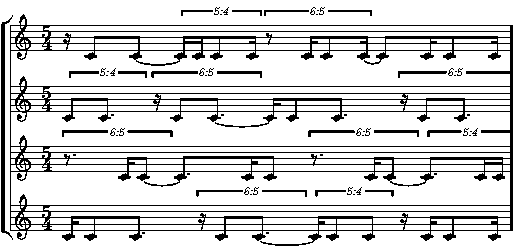
\includegraphics[scale=1.0]{images/abjad-6.pdf}


\begin{lstlisting}
>>> lower_staff = score['Lower Staff']
>>> show(lower_staff)
\end{lstlisting}

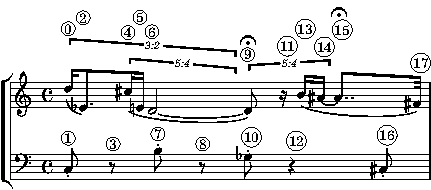
\includegraphics[scale=1.0]{images/abjad-7.pdf}


\begin{lstlisting}
>>> for note in iterate(lower_staff).by_class(Note):
...     attach(Articulation('staccato'), note)
... 
>>> show(score)
\end{lstlisting}

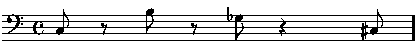
\includegraphics[scale=1.0]{images/abjad-8.pdf}


\begin{lstlisting}
>>> iterator = iterate(score).by_logical_tie(
...     nontrivial=True, pitched=True)
>>> for logical_tie in iterator:
...     attach(Fermata(), logical_tie.tail)
... 
>>> show(score)
\end{lstlisting}

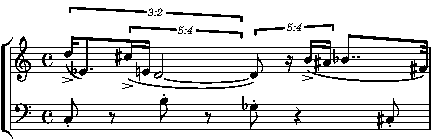
\includegraphics[scale=1.0]{images/abjad-9.pdf}


\begin{lstlisting}
>>> iterator = iterate(score).by_timeline()
>>> for index, component in enumerate(iterator):
...     markup = Markup(index, Up).circle()
...     attach(markup, component)
... 
>>> show(score)
\end{lstlisting}

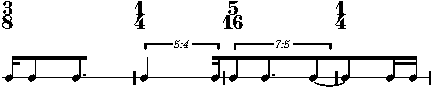
\includegraphics[scale=1.0]{images/abjad-10.pdf}


\section{Configuration}

We think it's important for composers to be able to define an operation (where
musical or notational) one time and be able to apply the operation to
arbitrarily many objects in the score at once. of the many ways abjad provides
of doing this, the most important (and most general) is iteration. examples
follow. iteration can be glossed as "define-once, apply-many". "configuration
reuse". we think it's important for composers to be able to configure objects a
single time, and then resuse the configuration as many times as necessary while
composing. we also think it's important to configure complex objects all at
once. "templating". we think it's important for composers to be able to
template all objects in the system, especially the hugely complex objects.
[JOSIAH]

\begin{lstlisting}
>>> rhythm_maker = rhythmmakertools.TaleaRhythmMaker(
...     talea=rhythmmakertools.Talea(
...         counts=(1, 2, 3),
...         denominator=16,
...         ),
...     )
>>> print(format(rhythm_maker))
rhythmmakertools.TaleaRhythmMaker(
    talea=rhythmmakertools.Talea(
        counts=(1, 2, 3),
        denominator=16,
        ),
    )
\end{lstlisting}


\begin{lstlisting}
>>> divisions = [(3, 8), (1, 4), (5, 16), (1, 4)]
>>> show(rhythm_maker, divisions=divisions)
\end{lstlisting}

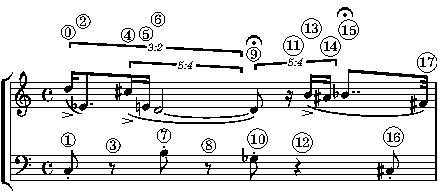
\includegraphics[scale=1.0]{images/abjad-11.pdf}


\begin{lstlisting}
>>> new_rhythm_maker = new(rhythm_maker,
...     talea__counts=(1, 2, 3, 4),
...     extra_counts_per_division=(0, 1),
...     )
>>> print(format(new_rhythm_maker))
rhythmmakertools.TaleaRhythmMaker(
    talea=rhythmmakertools.Talea(
        counts=(1, 2, 3, 4),
        denominator=16,
        ),
    extra_counts_per_division=(0, 1),
    )
\end{lstlisting}


\begin{lstlisting}
>>> show(new_rhythm_maker, divisions=divisions)
\end{lstlisting}

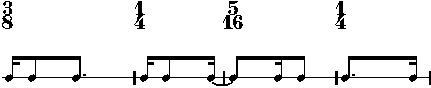
\includegraphics[scale=1.0]{images/abjad-12.pdf}


\begin{lstlisting}
>>> new_new_rhythm_maker = new(new_rhythm_maker,
...     extra_counts_per_division=(0, 1, 2),
...     beam_specifier=rhythmmakertools.BeamSpecifier(
...         beam_divisions_together=True,
...         ),
...     )
>>> print(format(new_new_rhythm_maker))
rhythmmakertools.TaleaRhythmMaker(
    talea=rhythmmakertools.Talea(
        counts=(1, 2, 3, 4),
        denominator=16,
        ),
    extra_counts_per_division=(0, 1, 2),
    beam_specifier=rhythmmakertools.BeamSpecifier(
        beam_each_division=True,
        beam_divisions_together=True,
        ),
    )
\end{lstlisting}


\begin{lstlisting}
>>> show(new_new_rhythm_maker, divisions=divisions)
\end{lstlisting}

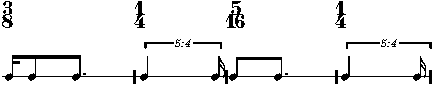
\includegraphics[scale=1.0]{images/abjad-13.pdf}


\section{Encapsulation}

We want everything to be encapsulated as much as possible. what this comes out
to mean is the system is overwhelming object-oriented (in the proper uses of
the term) and that all parts of the system (whether object-oriented or not) are
structured in such a way as to provide a single interface named according to a
uniform set of naming conventions. [TREVOR]

\section{Open-source best practices}

We try to follow the best practices of the open-source community (which has a
number of subpoints). [TREVOR]

\subsection{Extensibility}

As an open-source project, composers and researchers can contribute changes via
git pull requests. A process of continuous integration and online version
control simplifies this contribution process. 

\subsection{Embeddability}

Abjad is an importable Python library. It can be used in whole or in part as a
component of any Python-compatible system. Abjad has few Python package
dependencies and is not bound to any specific user application or graphic user
interface. These qualities make Abjad an ideal project ideal for embedding in
other software systems.

For example, Abjad supports IPython
Notebook\footnote{http://ipython.org/notebook.html}, a web-based interactive
computational environment combining code execution, text, mathematics, plots
and rich media into a single document. Notational output from Abjad can be
transparently captured and embedded directly into an IPython Notebook which has
loaded Abjad's IPython Notebook extension. Calls to Abjad's \texttt{show()} are
intercepted and the rendered graphics are embedded directly into the Notebook
along with the generating code. This allows scholars to quickly and intuitively
create music texts which can be shared, edited and executed by other IPython
users.

\subsection{Testability}

Text here.

\subsection{Maintainability}

Text here.

\section{conclusion}

we want composers to become programmers. for extremely good reasons. and the
priorities we have detailed here help make the case for why. [TREVOR]

\bibliography{tenor2015}
\end{document}